\section{Configurazione dell’architettura utilizzata}
Il processo di sperimentazione è stato svolto grazie all'utilizzo di macchine messe a disposizione da \textit{Reveal s.r.l}.
Il codice prodotto è stato prima eseguito su di un PC desktop domestico, per poi essere testato su un piccolo cluster di \clustersize{} macchine. Su di esse sono stati configurati ed installati l'ambiente Apache Spark, Spark NLP e Hadoop. Per testare la scalabilità offerta dal framework del John Snow Labs, il software è stato eseguito prima utilizzando soltanto una macchina per poi incrementare la potenza di calcolo a disposizione migrando l'esecuzione su di un sistema distribuito. 

\subsection{Hardware}
Le configurazioni delle macchine utilizzate sono le seguenti:\\
Configurazione macchina domestica:
\begin{itemize}
    \item Sistema operativo: Windows 10 Home
    \item Numero di CPU: 16
    \item Dimensione RAM: 16GB
\end{itemize}
Configurazione cluster (1 master, 2 workers):
\begin{itemize}
    \item Sistema operativo: CentOS 7
    \item Numero CPU per driver: 8
    \item Dimensione memoria per driver: 10 GB
    \item Numero di CPU per ogni worker: 4
    \item Dimensione memoria per ogni worker: 10 GB
\end{itemize}

\subsection{Software}
Come citato precedentemente, l'obiettivo è quello di testare soluzioni per la risoluzione di task di NLP in ambiente distribuito, confrontando i risultati ottenuti in termini di accuratezza e tempi di esecuzione. Per eseguire l'applicazione, all'interno del sistema sono stati configurati: l'ambiente Spark, un database distribuito HDFS ed il resource manager YARN. 

Nella macchina master risiedono il driver di Spark, il \textbf{NameNode} (deamon per HDFS), responsabile della gestione del namespace del file system e il \textbf{ResourceManager} (deamon per YARN), responsabile dell’assegnazione e della gestione delle risorse tra tutte le applicazioni. Quando Spark NLP richiede al sistema l'esecuzione di un job o di un DAG di jobs, questa richiesta viene inoltrata all'istanza di YARN in esecuzione sul nodo master che verifica se l'esecuzione è possibile e, in caso affermativo, registra l'applicazione assegnandogli un Job ID e aggiungendolo alla coda dei job da eseguire. 

Ogni volta che un job viene estratto dalla coda ed è mandato in esecuzione, il ResourceManager seleziona casualmente un DataNode (processo di HDFS) e avvia su quello stesso nodo un processo ApplicationMaster (processo di YARN). Al passo successivo, l'ApplicationMaster comunicherà con il NameNode che a sua volta si occuperà di accertarsi della posizione in cui si trovano i file (blocchi) all'interno del cluster e di quante risorse ha bisogno il job. 

Una volta svolte tutte le valutazioni, l'ApplicationMaster invia le informazioni sulla richiesta di risorse al ResourceManager che le esamina e inoltra una richiesta di allocazione di queste, sotto forma di container, ai nodi del cluster. Questi container sono detti \textit{Esecutori}. I NodeManager di ogni singolo nodo worker si occuperanno quindi di allocare le risorse come da richiesta del ResourceManager. 

Infine, gli esecutori inizieranno l'esecuzione dei job a loro assegnati e proseguiranno la comunicazione direttamente con il programma driver (SparkContext). L'output sarà direttamente restituito al client.

Sul cluster utilizzato in questo progetto, l'applicazione è stata eseguita nella cosiddetta \textit{Client Mode}, ovvero, il driver Spark viene avviato sulla stessa macchina da cui viene inviata l'applicazione.

\begin{figure}[hbt!]
    \centering
    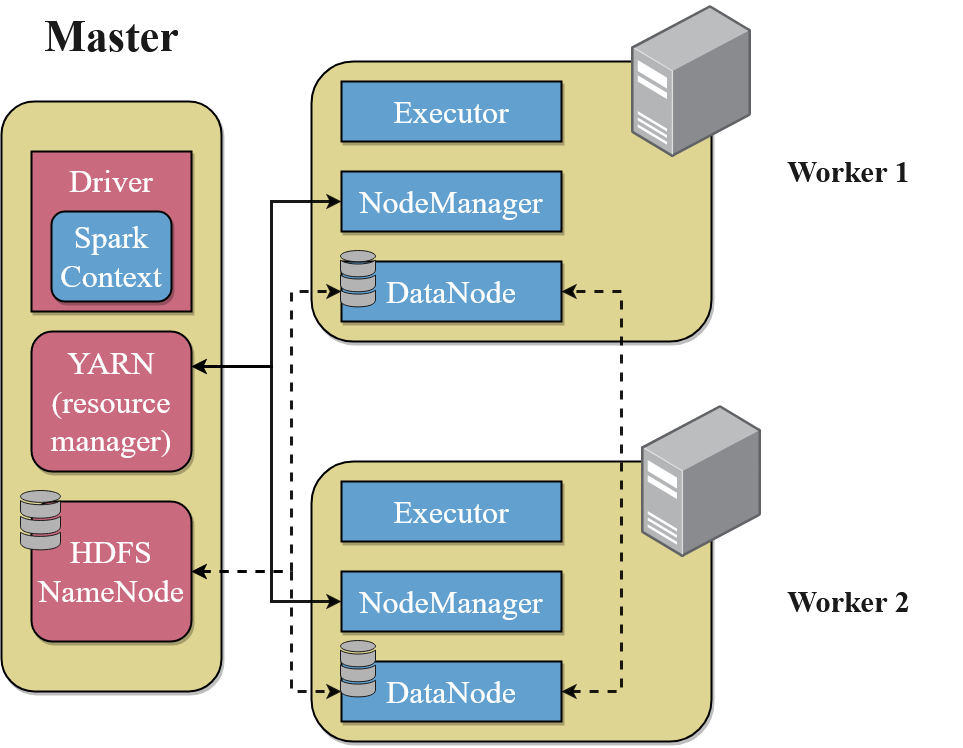
\includegraphics[width=1\textwidth]{img/architecture/cluster_architecture2.png}
    \caption{Architettura del cluster}
    \label{fig:cluster_architecture}
\end{figure}

\begin{figure}[hbt!]
    \centering
    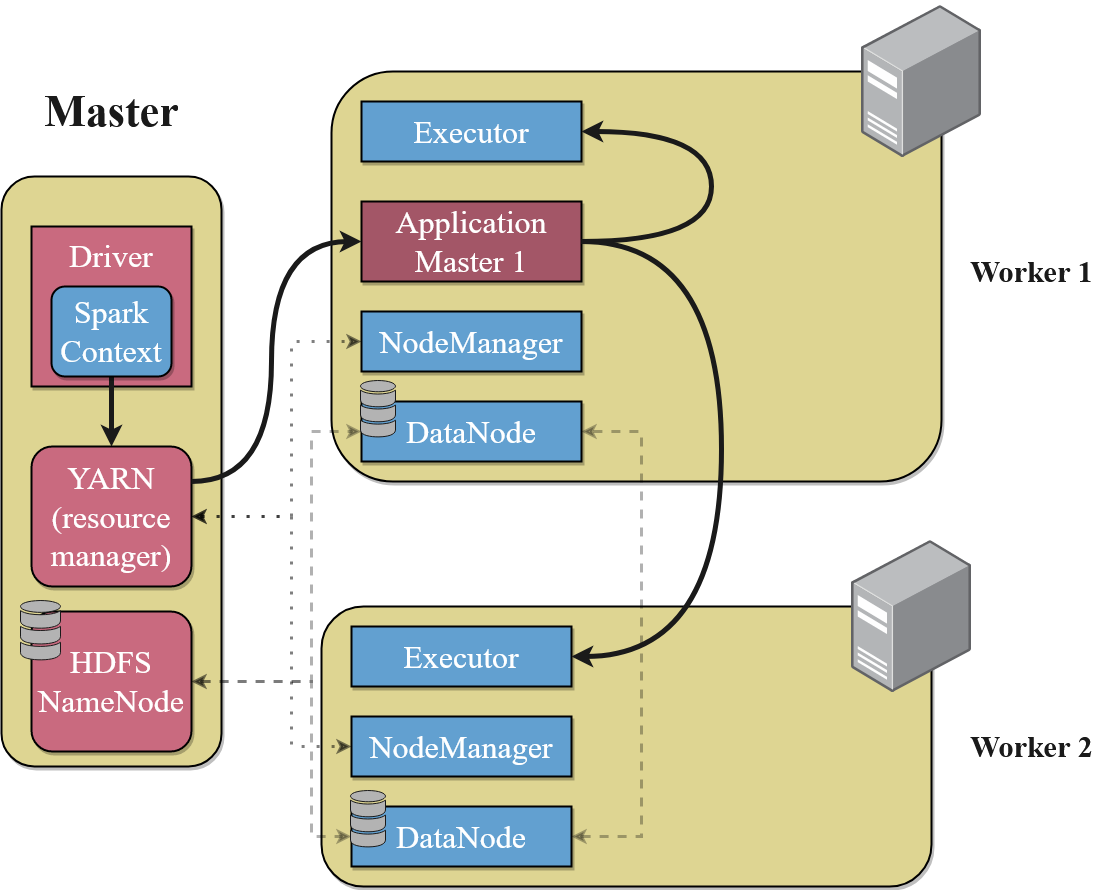
\includegraphics[width=0.7\textwidth]{img/architecture/application_submit2.png}
    \caption{Richiesta di esecuzione dell'applicazione}
    \label{fig:application_submit}
\end{figure}

\begin{figure}[hbt!]
    \centering
    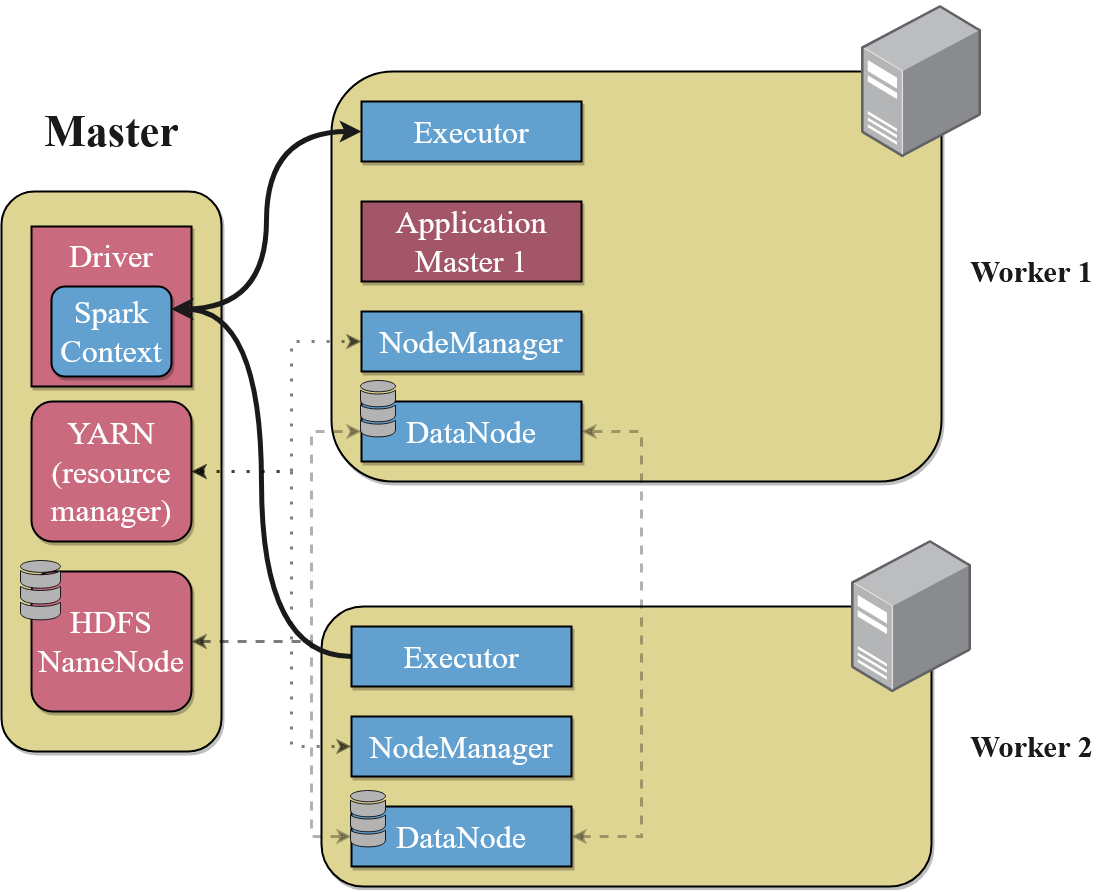
\includegraphics[width=0.7\textwidth]{img/architecture/jobs_execution2.png}
    \caption{Esecuzione dei compiti: interazione tra esecutori e driver}
    \label{fig:jobs_execution}
\end{figure}

